\begin{proofbox}
\par\medskip
\begin{minipage}{\linewidth}
\par\medskip
\begin{minipage}{\linewidth}
\noindent
\textbf{\textcolor{CProof}{证明一｜最快证明法（考场速写，推荐）}}\par\nobreak\smallskip
\par
\begin{minipage}{\linewidth}
\begin{center}
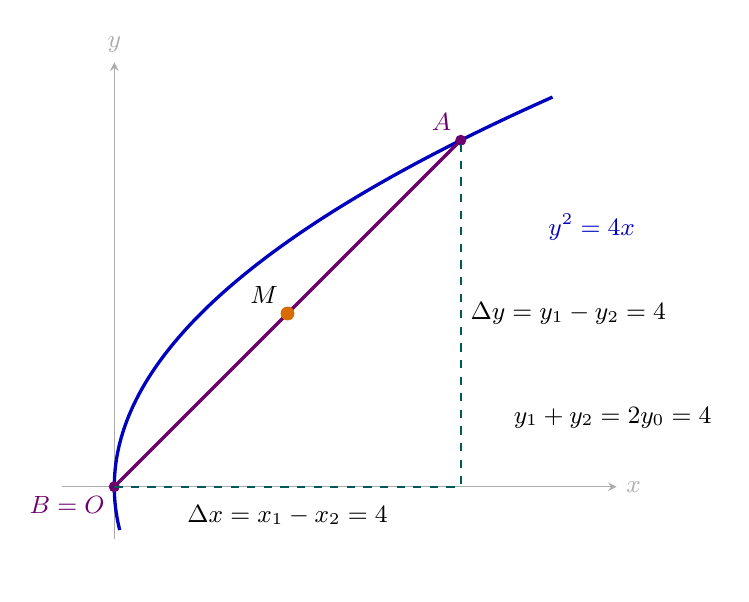
\begin{tikzpicture}[x=1.1cm,y=1.1cm,>=stealth,font=\small]
\path[use as bounding box] (-1,-1) rectangle (7,5.3);
\draw[->,gray!65] (-.6,0)--(5.8,0) node[right] {$x$};
\draw[->,gray!65] (0,-.6)--(0,4.9) node[above] {$y$};
\draw[blue!75!black,very thick,domain=-.5:4.5,samples=100,variable=\v] plot ({\v*\v/4},\v);
\draw[violet!85!black,very thick] (0,0)--(4,4);
\fill[violet!85!black] (4,4) circle(2pt) node[above left] {$A$};
\fill[violet!85!black] (0,0) circle(2pt) node[below left] {$B=O$};
\fill[orange!85!black] (2,2) circle(2.5pt);
\node[blue!75!black,right] at (4.9,3) {$y^2=4x$};

\node[above left] at (2,2) {$M$};
\draw[teal!70!black,dashed,thick] (0,0)--(4,0)--(4,4);
\node[below] at (2,-.1) {$\Delta x=x_1-x_2=4$};
\node[right] at (4,2) {$\Delta y=y_1-y_2=4$};
\node[right] at (4.5,.8) {$y_1+y_2=2y_0=4$};
\end{tikzpicture}
\par\small 横纵差构成斜率；纵标和等于中点纵标的两倍。
\end{center}
\end{minipage}\par
\end{minipage}
\par

\par

\end{minipage}


\par\noindent\textbf{识别信号：}“抛物线 + 弦中点 + 求斜率”。
\par\noindent\textbf{优势：}只用平方差与中点公式，二至三步结束。
设 $A(x_1,y_1),B(x_2,y_2)$ 为不同的交点，$M(x_0,y_0)$ 为中点。因为两点在 $y^2=2px$ 上，
\[
\begin{aligned}
 (y_1-y_2)(y_1+y_2)&=2p(x_1-x_2),\\
 k_{AB}=\frac{y_1-y_2}{x_1-x_2}
 &=\frac{2p}{y_1+y_2}
 =\boxed{\frac{p}{y_0}}.
\end{aligned}
\]
其中 $x_1\ne x_2$ 才能写有限斜率；原式保证此时 $y_1+y_2=2y_0\ne0$。
\par\smallskip
\par\noindent\textbf{记忆负担最小的线索：}“\textbf{两点作差}\ $\to$\ \textbf{平方差}\ $\to$\ \textbf{纵标求和} $2y_0$”。
\par\medskip
\begin{minipage}{\linewidth}
\par\medskip
\begin{minipage}{\linewidth}
\noindent
\textbf{\textcolor{CProof}{证明二｜最低门槛法（中点对称设点，只设一个 $t$）}}\par\nobreak\smallskip
\par
\begin{minipage}{\linewidth}
\begin{center}
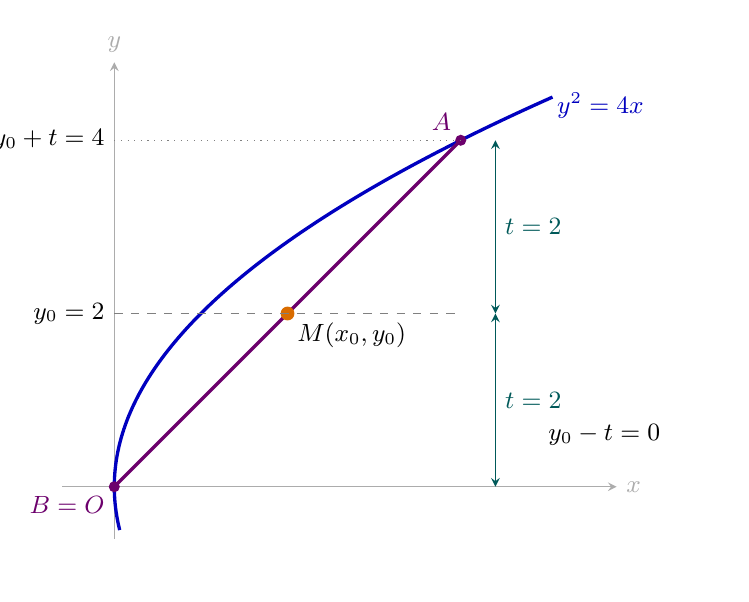
\begin{tikzpicture}[x=1.1cm,y=1.1cm,>=stealth,font=\small]
\path[use as bounding box] (-1,-1) rectangle (7,5.3);
\draw[->,gray!65] (-.6,0)--(5.8,0) node[right] {$x$};
\draw[->,gray!65] (0,-.6)--(0,4.9) node[above] {$y$};
\draw[blue!75!black,very thick,domain=-.5:4.5,samples=100,variable=\v] plot ({\v*\v/4},\v);
\draw[violet!85!black,very thick] (0,0)--(4,4);
\fill[violet!85!black] (4,4) circle(2pt) node[above left] {$A$};
\fill[violet!85!black] (0,0) circle(2pt) node[below left] {$B=O$};
\fill[orange!85!black] (2,2) circle(2.5pt);
\node[blue!75!black,right] at (5,4.4) {$y^2=4x$};

\node[below right] at (2,2) {$M(x_0,y_0)$};
\draw[gray,dashed] (0,2)--(4,2);
\draw[<->,teal!70!black] (4.4,2)--(4.4,4) node[midway,right] {$t=2$};
\draw[<->,teal!70!black] (4.4,0)--(4.4,2) node[midway,right] {$t=2$};
\node[left] at (0,4) {$y_0+t=4$};
\node[left] at (0,2) {$y_0=2$};
\draw[gray,dotted] (0,4)--(4,4);
\node[right] at (4.9,.6) {$y_0-t=0$};
\end{tikzpicture}

\par\small 两端点纵坐标在 $y_0$ 两侧等距展开。
\end{center}
\end{minipage}\par
\end{minipage}
\par

\par

\end{minipage}


\par\noindent\textbf{为什么选它：}不必记抽象公式，更不必同时设 $x_1,x_2,y_1,y_2$；一眼看出中点的作用。
\begin{description}[style=nextline,leftmargin=2.8em,labelsep=0.5em,itemsep=0.35em]
 \item[\textbf{步骤1（先固定纵坐标）：}] 设 $A,B$ 的纵坐标分别为 $y_0+t$ 与 $y_0-t$，$t\ne0$（不同点，故纵坐标必不同）。
 \item[\textbf{步骤2（由曲线直接写横坐标）：}] 两个横坐标为
 \[x_A=\frac{(y_0+t)^2}{2p},\qquad x_B=\frac{(y_0-t)^2}{2p}.\]
 \item[\textbf{步骤3（只求差，不求端点）：}]
 \[
 \Delta y=2t,\qquad
 \Delta x=\frac{(y_0+t)^2-(y_0-t)^2}{2p}
 =\frac{2y_0t}{p}.
 \]
 \item[\textbf{步骤4（斜率 = 纵差/横差）：}]
 \[k=\frac{\Delta y}{\Delta x}=\frac{2t}{2y_0t/p}=\boxed{\frac{p}{y_0}}.\]
\end{description}
\par\noindent\textbf{理解加分：}$\Delta x\propto y_0$，所以 $y_0=0$ 时两端点的横坐标相同，弦正是\textbf{竖直}的；没有“无穷大斜率”这种实数值可代入公式。
\par\medskip
\begin{minipage}{\linewidth}
\noindent
\textbf{\textcolor{CProof}{深挖｜相减为何看方向，相加为何看长度？（圆与抛物线同构）}}\par\nobreak\smallskip
\par\noindent\textbf{第1步：先问我们究竟想求什么。}\par\nobreak\smallskip\par
\end{minipage}
\par

已知中点 $M$，端点只能写作 $A=M+(u,t)$、$B=M-(u,t)$。未知 $u,t$ 有两类信息：
\textbf{方向}由比值 $t/u$ 决定；\textbf{远近}由 $\sqrt{u^2+t^2}$ 决定。因而自然寻找\textbf{一条线性的方向关系}和\textbf{一条平方的长度关系}。


\par
\begin{minipage}{\linewidth}
\begin{center}
% 解析坐标严格确定：圆 x^2+y^2=25，A=(3,4), B=(3,-4), M=(3,0)
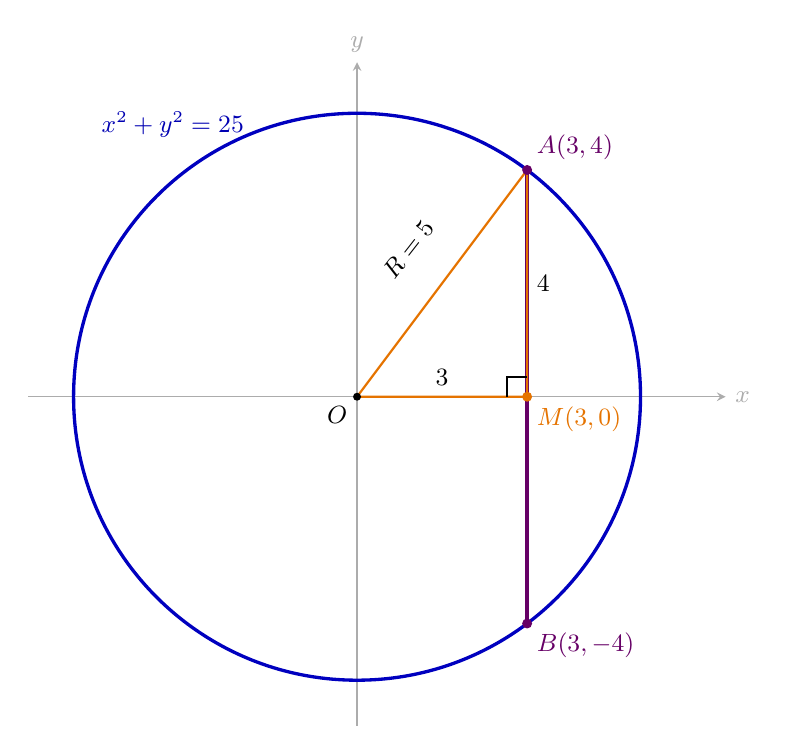
\begin{tikzpicture}[scale=.72,>=stealth,font=\small]
  \draw[->,gray!65] (-5.8,0)--(6.5,0) node[right] {$x$};
  \draw[->,gray!65] (0,-5.8)--(0,5.9) node[above] {$y$};
  \draw[very thick,blue!75!black] (0,0) circle (5);
  \draw[very thick,violet!80!black] (3,-4)--(3,4);
  \draw[thick,orange!90!black] (0,0)--(3,0)--(3,4)--cycle;
  \draw[black,thick] (2.65,0)--(2.65,.35)--(3,.35);
  \fill[black] (0,0) circle(2pt) node[below left] {$O$};
  \fill[orange!90!black] (3,0) circle(2.5pt) node[below right] {$M(3,0)$};
  \fill[violet!80!black] (3,4) circle(2.5pt) node[above right] {$A(3,4)$};
  \fill[violet!80!black] (3,-4) circle(2.5pt) node[below right] {$B(3,-4)$};
  \node[above] at (1.5,0.03) {$3$};
  \node[right] at (3,2.0) {$4$};
  \node[rotate=52] at (0.9,2.6) {$R=5$};
  \node[blue!70!black] at (-3.25,4.8) {$x^2+y^2=25$};
\end{tikzpicture}

\par\small 圆中 $OM\perp AB$，直角三角形 $OMA$ 给出半弦长。
\end{center}
\end{minipage}
\par

\par\noindent\textbf{第2步：先用圆作标准参照。}\par\nobreak\smallskip
圆 $x^2+y^2=R^2$ 上的两端点满足
\[
\begin{cases}
(x_0+u)^2+(y_0+t)^2=R^2,\\
(x_0-u)^2+(y_0-t)^2=R^2.
\end{cases}
\]
相减得 $4(x_0u+y_0t)=0$，即 $OM\perp AB$（$M\ne O$）；相加得
$2(x_0^2+y_0^2+u^2+t^2)=2R^2$，即
\[
\underbrace{OM^2}_{\text{中点离圆心多远}}
+\underbrace{AM^2}_{\text{半弦长平方}}
=\underbrace{R^2}_{\text{半径平方}}.
\]

\par
\begin{minipage}{\linewidth}
\begin{center}
% 精确数值：y²=4x, p=2, A(9,6), B(1,-2), M(5,2), T(1,2), 半位移 (u,t)=(4,4)
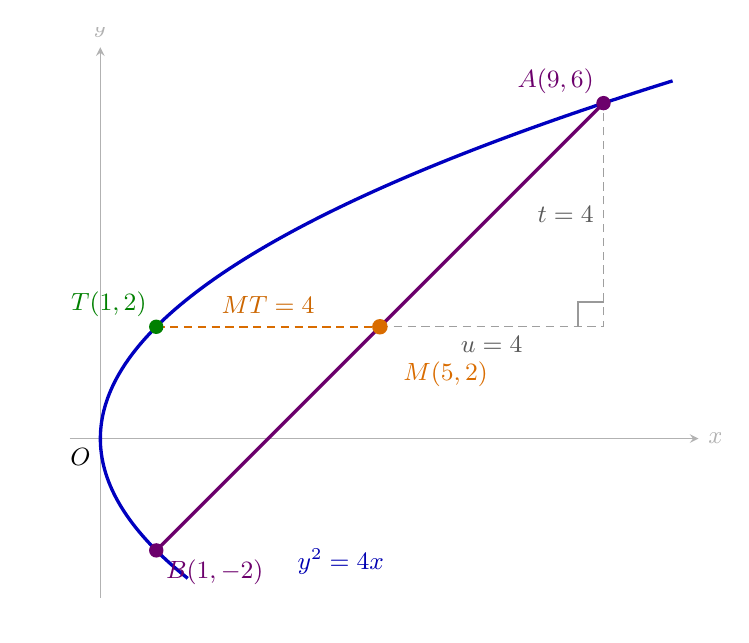
\begin{tikzpicture}[x=.71cm,y=.71cm,>=stealth,font=\small]
  \clip (-1.3,-3.15) rectangle (11.1,7.35);
  \draw[->,gray!60] (-.55,0)--(10.7,0) node[right] {$x$};
  \draw[->,gray!60] (0,-2.85)--(0,7.0) node[above] {$y$};
  \draw[blue!75!black,very thick,samples=125,domain=-2.5:6.4,variable=\v,smooth]
    plot ({\v*\v/4},{\v});
  \draw[violet!85!black,very thick] (1,-2)--(9,6);
  \draw[densely dashed,orange!85!black,thick] (1,2)--(5,2);
  \draw[gray!75,densely dashed] (5,2)--(9,2)--(9,6);
  \fill[violet!85!black] (9,6) circle (2.6pt) node[above left] {$A(9,6)$};
  \fill[violet!85!black] (1,-2) circle (2.6pt) node[below right] {$B(1,-2)$};
  \fill[orange!85!black] (5,2) circle (2.8pt) node[below right,xshift=5pt,yshift=-9pt] {$M(5,2)$};
  \fill[green!50!black] (1,2) circle (2.6pt) node[above left] {$T(1,2)$};
  \draw[gray!80,thick] (8.55,2)--(8.55,2.45)--(9,2.45);
  \node[above,orange!80!black] at (3.0,2.07) {$MT=4$};
  \node[below,gray!70!black] at (7.0,2) {$u=4$};
  \node[left,gray!70!black] at (9,4.0) {$t=4$};
  \node[blue!70!black] at (4.3,-2.2) {$y^2=4x$};
  \node[below left] at (0,0) {$O$};
\end{tikzpicture}

\par\small 抛物线：半位移 $(u,t)$ 给方向，直角三角形给实际半弦长。
\end{center}
\end{minipage}
\par

\par\noindent\textbf{第3步：换成抛物线。}\par\nobreak\smallskip
方程 $y^2=2px$ 给出
\[
\begin{cases}
(y_0+t)^2=2p(x_0+u),\\
(y_0-t)^2=2p(x_0-u).
\end{cases}
\]
\textbf{相减}：$4y_0t=4pu\Rightarrow\boxed{y_0t=pu}$，因此非竖直时 $k=t/u=p/y_0$。
\textbf{相加}：$2(y_0^2+t^2)=4px_0\Rightarrow\boxed{t^2=2px_0-y_0^2}$，因此判定弦是否存在及纵向半跨度。

\par\noindent\textbf{第4步：补齐真正的弦长。}\par\nobreak\smallskip
相减给 $u=y_0t/p$，相加给 $t^2$；两者一起代入\textbf{直角三角形的勾股定理}：
\[
\boxed{\displaystyle AB=2\sqrt{u^2+t^2}
 =2\sqrt{(2px_0-y_0^2)\!\left(1+\frac{y_0^2}{p^2}\right)}}.
\]
\par\noindent\textbf{辨析：}圆中“相加”直接得到勾股；抛物线中“相加”得到 $t^2$，\textbf{再组合方向信息才得到真正的弦长勾股}，不能把 $t^2=2px_0-y_0^2$ 说成普通三角形勾股。


\par
\begin{minipage}{\linewidth}
\begin{center}
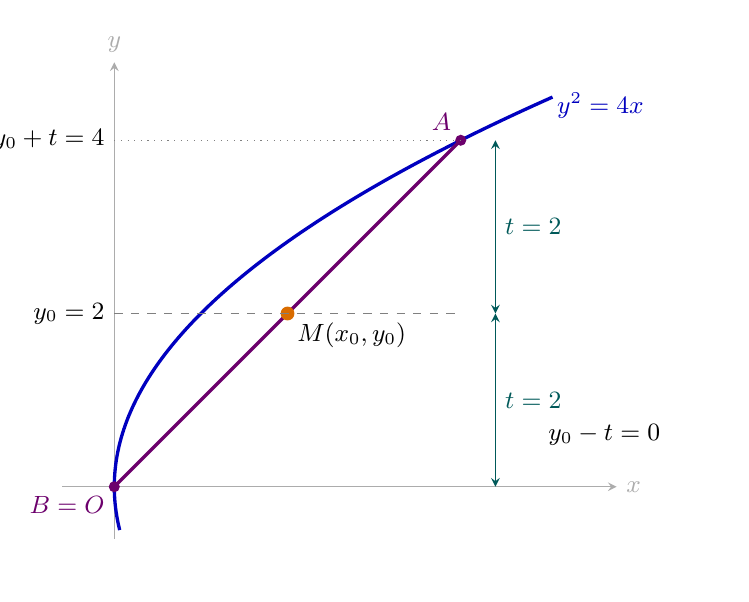
\begin{tikzpicture}[x=1.1cm,y=1.1cm,>=stealth,font=\small]
\path[use as bounding box] (-1,-1) rectangle (7,5.3);
\draw[->,gray!65] (-.6,0)--(5.8,0) node[right] {$x$};
\draw[->,gray!65] (0,-.6)--(0,4.9) node[above] {$y$};
\draw[blue!75!black,very thick,domain=-.5:4.5,samples=100,variable=\v] plot ({\v*\v/4},\v);
\draw[violet!85!black,very thick] (0,0)--(4,4);
\fill[violet!85!black] (4,4) circle(2pt) node[above left] {$A$};
\fill[violet!85!black] (0,0) circle(2pt) node[below left] {$B=O$};
\fill[orange!85!black] (2,2) circle(2.5pt);
\node[blue!75!black,right] at (5,4.4) {$y^2=4x$};

\node[below right] at (2,2) {$M(x_0,y_0)$};
\draw[gray,dashed] (0,2)--(4,2);
\draw[<->,teal!70!black] (4.4,2)--(4.4,4) node[midway,right] {$t=2$};
\draw[<->,teal!70!black] (4.4,0)--(4.4,2) node[midway,right] {$t=2$};
\node[left] at (0,4) {$y_0+t=4$};
\node[left] at (0,2) {$y_0=2$};
\draw[gray,dotted] (0,4)--(4,4);
\node[right] at (4.9,.6) {$y_0-t=0$};
\end{tikzpicture}

\par\small 以 $M$ 为中心交换 $A,B$，位移 $+t$ 与 $-t$ 交换，平方不变。
\end{center}
\end{minipage}
\par

\par\noindent\textbf{第5步：用一条式子统一两种运算（进阶可选）。}\par\nobreak\smallskip
设 $F(x,y)=y^2-2px$，并记
$F(M\pm(u,t))=0$，则展开为
\[
\boxed{F(M\pm(u,t))=
 \underbrace{(y_0^2-2px_0+t^2)}_{\text{偶项：相加保留}}
 \ \pm\ \underbrace{(2y_0t-2pu)}_{\text{奇项：相减保留}}}.
\]
两个端点都在曲线上意味着两个括号\textbf{分别为零}。这解释了为什么任何这种关于中点的\textbf{二次曲线}，加减两式都有明确的几何分工。
\par\medskip
\begin{minipage}{\linewidth}
\par\medskip
\begin{minipage}{\linewidth}
\noindent
\textbf{\textcolor{CProof}{证明三｜常规方法（联立直线 + 韦达定理）}}\par\nobreak\smallskip
\par
\begin{minipage}{\linewidth}
\begin{center}
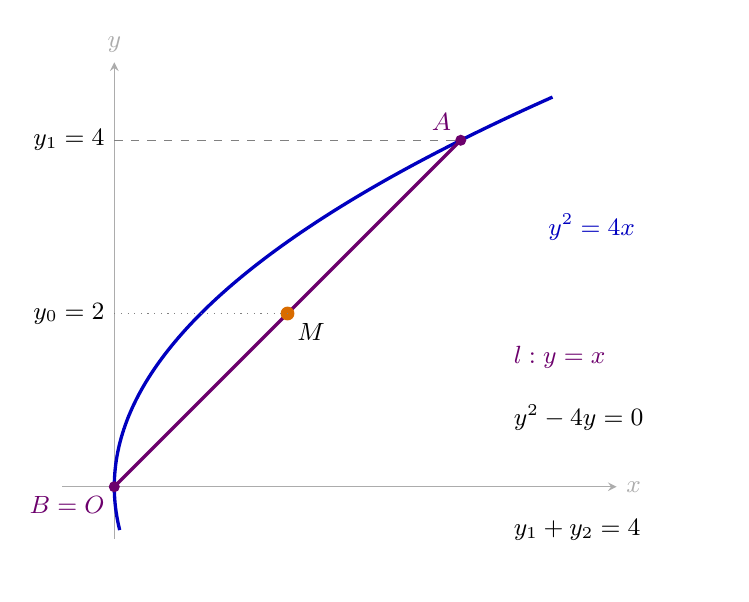
\begin{tikzpicture}[x=1.1cm,y=1.1cm,>=stealth,font=\small]
\path[use as bounding box] (-1,-1) rectangle (7,5.3);
\draw[->,gray!65] (-.6,0)--(5.8,0) node[right] {$x$};
\draw[->,gray!65] (0,-.6)--(0,4.9) node[above] {$y$};
\draw[blue!75!black,very thick,domain=-.5:4.5,samples=100,variable=\v] plot ({\v*\v/4},\v);
\draw[violet!85!black,very thick] (0,0)--(4,4);
\fill[violet!85!black] (4,4) circle(2pt) node[above left] {$A$};
\fill[violet!85!black] (0,0) circle(2pt) node[below left] {$B=O$};
\fill[orange!85!black] (2,2) circle(2.5pt);
\node[blue!75!black,right] at (4.9,3) {$y^2=4x$};

\node[below right] at (2,2) {$M$};
\draw[gray,dashed] (0,4)--(4,4);
\node[left] at (0,4) {$y_1=4$};
\node[left] at (0,2) {$y_0=2$};
\draw[gray,dotted] (0,2)--(2,2);
\node[right,violet!85!black] at (4.5,1.5) {$l:y=x$};
\node[right] at (4.5,.8) {$y^2-4y=0$};
\node[right] at (4.5,-.5) {$y_1+y_2=4$};
\end{tikzpicture}

\par\small 交点的两个纵坐标，就是消去 $x$ 后方程的两个根。
\end{center}
\end{minipage}\par
\end{minipage}
\par

\par

\end{minipage}


\par\noindent\textbf{为什么要有它：}考试如果还要找交点、判别式、弦长或处理中点轨迹，此法直接衔接完整解析几何流程。
设弦所在直线为 $y=kx+b$。由于非退化水平直线与 $y^2=2px$ 至多只有一个交点，真正的非竖直弦必有 $k\ne0$。写作
\[x=\frac{y-b}{k},\]
代入 $y^2=2px$ 得
\[
 y^2=\frac{2p}{k}(y-b)
 \quad\Longleftrightarrow\quad
 y^2-\frac{2p}{k}y+\frac{2pb}{k}=0.
\]
该一元二次方程的两个不同实根是 $y_1,y_2$。由韦达定理
\[
 \begin{aligned}
 y_1+y_2&=\frac{2p}{k},\\
 y_0=\frac{y_1+y_2}{2}&=\frac{p}{k}
 \quad\Longrightarrow\quad\boxed{k=\frac{p}{y_0}}.
 \end{aligned}
\]
\par\noindent\textbf{成立条件：}判别式必须 $>0$ 才有两个不同实交点；若判别式 $=0$，得到的是切线而非非退化弦。
\par\medskip
\begin{minipage}{\linewidth}
\par\medskip
\begin{minipage}{\linewidth}
\noindent
\textbf{\textcolor{CProof}{补充四｜存在性的严格证明（“反用公式”时必须补）}}\par\nobreak\smallskip
\par
\begin{minipage}{\linewidth}
\begin{center}
\begin{tikzpicture}[x=.95cm,y=.95cm,>=stealth,font=\small]
\foreach \s/\m/\d/\title in {0/2/4/{D>0},4.5/1/0/{D=0},9/0/{-4}/{D<0}} {
 \begin{scope}[shift={(\s,0)}]
 \path[use as bounding box] (-.5,-.7) rectangle (4.1,5.4);
 \draw[->,gray!65] (-.3,0)--(3.6,0) node[right] {$x$};
 \draw[->,gray!65] (0,-.3)--(0,4.9);
 \draw[blue!75!black,thick,domain=0:4.1,samples=70,variable=\v] plot ({\v*\v/4},\v);
 \draw[violet!85!black,thick,dashed,domain=0:{2.1+\m},variable=\q] plot ({\q},{\q+2-\m});
 \fill[orange!85!black] (\m,2) circle(2.5pt) node[below right] {$M$};
 \node at (1.5,5.1) {$\title$};
 \node at (1.5,-.6) {$M(\m,2)$};
 \end{scope}
}
\fill[violet!85!black] (0,0) circle(2pt);
\fill[violet!85!black] (4,4) circle(2pt);
\fill[violet!85!black] (5.5,2) circle(2pt);
\node at (1.5,4.4) {两个不同实端点};
\node at (6,4.4) {两端点重合};
\node at (10.5,4.4) {无实交点};
\end{tikzpicture}
\par\small 同尺度比较：固定 $y_0=2$，改变 $x_0$；$D=4x_0-4$。
\end{center}
\end{minipage}\par
\end{minipage}
\par

\par

\end{minipage}


沿用方法二中的 $y_A=y_0+t,\;y_B=y_0-t$，由中点横坐标定义：
\[
 x_0=\frac{x_A+x_B}{2}
 =\frac{(y_0+t)^2+(y_0-t)^2}{4p}
 =\frac{y_0^2+t^2}{2p}.
\]
故
\[\boxed{t^2=2px_0-y_0^2}.\]
\par\noindent\textbf{必要性：}若 $A\ne B$ 是实点，则 $t\ne0$，故 $2px_0-y_0^2=t^2>0$。
\par\noindent\textbf{充分性：}若 $2px_0-y_0^2>0$，取 $t=\sqrt{2px_0-y_0^2}>0$，令
\[
 A\left(\frac{(y_0+t)^2}{2p},y_0+t\right),\quad
 B\left(\frac{(y_0-t)^2}{2p},y_0-t\right).
\]
它们确实是曲线上\textbf{两个不同实点}，且其中点是 $M(x_0,y_0)$，因此条件充分。这样的两个端点（互换顺序视为相同）也是唯一的。
\par\smallskip
\par\noindent\textbf{边界分类：}
\begin{itemize}[leftmargin=*,itemsep=0.2em]
 \item $2px_0>y_0^2,\ y_0\ne0$：非竖直弦，$k=p/y_0$。
 \item $2px_0>y_0^2,\ y_0=0$：竖直弦 $x=x_0$，斜率不存在。
 \item $2px_0=y_0^2$：$t=0$，只得到重合端点；切线存在，但\textbf{不存在非退化弦}。
 \item $2px_0<y_0^2$：$t^2<0$，不存在实弦。
\end{itemize}
\par\medskip
\begin{minipage}{\linewidth}
\par\medskip
\begin{minipage}{\linewidth}
\noindent
\textbf{\textcolor{CProof}{补充五｜导数视角（帮助理解，不作为必背证明）}}\par\nobreak\smallskip
\par
\begin{minipage}{\linewidth}
\begin{center}
\begin{tikzpicture}[x=1.1cm,y=1.1cm,>=stealth,font=\small]
\path[use as bounding box] (-1,-1) rectangle (7,5.3);
\draw[->,gray!65] (-.6,0)--(5.8,0) node[right] {$x$};
\draw[->,gray!65] (0,-.6)--(0,4.9) node[above] {$y$};
\draw[blue!75!black,very thick,domain=-.5:4.5,samples=100,variable=\v] plot ({\v*\v/4},\v);
\draw[violet!85!black,very thick] (0,0)--(4,4);
\fill[violet!85!black] (4,4) circle(2pt) node[above left] {$A$};
\fill[violet!85!black] (0,0) circle(2pt) node[below left] {$B=O$};
\fill[orange!85!black] (2,2) circle(2.5pt);
\node[blue!75!black,right] at (4.9,3) {$y^2=4x$};

\draw[green!50!black,thick,dashed] (-.4,.6)--(3.9,4.9);
\draw[gray,dotted] (1,2)--(2,2);
\fill[green!50!black] (1,2) circle(2.5pt) node[above left] {$T(1,2)$};
\node[below right,orange!85!black] at (2,2) {$M(2,2)$};
\node[right,green!50!black] at (4.7,1.3) {$\text{切线 }y=x+1$};
\node[right] at (4.7,.5) {$k_T=k_{AB}=1$};
\end{tikzpicture}
\par\small 同纵标曲线点 $T$ 处的切线与弦平行；$M$ 不是切点。
\end{center}
\end{minipage}\par
\end{minipage}
\par

\par

\end{minipage}


由 $y^2=2px$ 对 $x$ 求导：$2y\,y'=2p$，故曲线上 $y=y_0\ne0$ 的点 $T$ 处，切线斜率为 $p/y_0$。与方法一的结果相同，所以\textbf{中点弦方向等于曲线上“同纵坐标点”的切线方向}。千万不要把中点 $M$ 当作切点。
\par\medskip
\begin{minipage}{\linewidth}
\noindent
\textbf{\textcolor{CProof}{最终结论}}\par\nobreak\smallskip
\[\boxed{\displaystyle k_{AB}=\frac{p}{y_0}\quad\text{（非竖直真实弦）}}\]\par
\end{minipage}
\par

考场首选\textbf{证明一}；初学理解首选\textbf{证明二}；涉及交点和判别式首选\textbf{证明三}；由指定中点反求弦要加\textbf{存在性验证}。
\end{proofbox}
